\section{Post-hoc accounting of the saved run}

This section is post-hoc. It was computed on 2026-09-14 from the saved forecasts after the registered
results were seen, adds no test, and does not change the status of anything above. Each window's \qs{} is
split exactly into three parts, each divided by the full horizon: the loss on zero-target days, which for
nonnegative quantiles is $\frac{2}{9h}\sum_{y_t = 0}\sum_\tau (1-\tau) q_{t,\tau}$; the loss on positive days
from quantiles above the target (overprediction); and the loss on positive days from quantiles below it
(underprediction). The parts sum to \qs{} on all 48,600 rows to floating-point tolerance, and the same
within-repository and across-repository averaging reproduces the 18 registered mean differences. The
decomposition locates where a loss difference arises; it says nothing about why a model forecast what it did.

\begin{table}[t]
\centering\small
\caption{Post-hoc. The mean difference against \lm{} and its three parts, model minus reference; negative
favors the model. The parts sum to the total.}
\label{tab:posthoc}
\begin{tabular}{llrrrr}
\toprule
Model & $h$ & Total & Zero days & Positive, overprediction & Positive, underprediction \\
\midrule
Chronos-2 & 7 & -0.137 & 0.005 & -0.095 & -0.048 \\
Chronos-2 & 30 & -0.132 & 0.005 & -0.156 & 0.019 \\
Chronos-2 & 90 & -0.101 & 0.004 & -0.184 & 0.078 \\
TimesFM 3 & 7 & -0.258 & 0.004 & -0.091 & -0.171 \\
TimesFM 3 & 30 & -0.201 & 0.006 & -0.150 & -0.057 \\
TimesFM 3 & 90 & -0.128 & 0.011 & -0.187 & 0.047 \\
TimesFM 2.5 & 7 & -0.243 & 0.012 & -0.088 & -0.167 \\
TimesFM 2.5 & 30 & -0.201 & 0.014 & -0.163 & -0.052 \\
TimesFM 2.5 & 90 & -0.112 & 0.015 & -0.209 & 0.082 \\
\bottomrule
\end{tabular}
\end{table}

Table~\ref{tab:posthoc} gives the parts for the nine cells against the local mean. The finding in one
sentence: the mean gain sits on positive days where the local mean overpredicts, and the zero-day part is
small beside it. The zero-day part is positive, against the models, in every cell, from 0.004 to 0.015: small
beside mean differences of $-0.101$ to $-0.258$, but in every cell larger than that cell's median
difference in Table~\ref{tab:lm}, where the medians run from 0.0003 to 0.0041. The overprediction part favors the models in every cell,
from $-0.088$ to $-0.209$. The underprediction part favors the models at 7 days, where for both TimesFM
models it is the larger of the two positive-day parts, and favors the local mean at 90 days, where the
models' underprediction loss exceeds the local mean's. Why the local mean overpredicts on those days is not
something the accounting tests.

\begin{figure}[t]
\centering
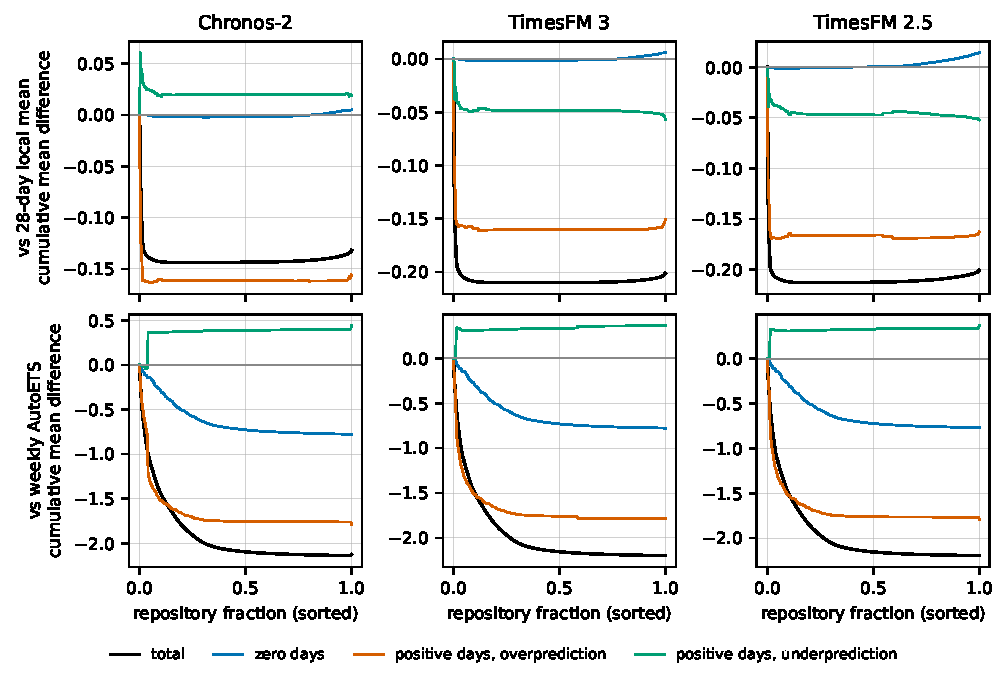
\includegraphics[width=\textwidth]{fig-posthoc-cumulative-h30}
\caption{Post-hoc. Signed cumulative contribution to the mean difference at horizon 30, repositories sorted
by their total difference (ascending) and the cumulative sum divided by 300, so each curve ends at its mean.
Top row: against \lm{}; bottom row: against \aets{}. Vertical scales differ between rows.}
\label{fig:cumulative}
\end{figure}

Figure~\ref{fig:cumulative} shows the same accounting as cumulative curves. Against the local mean, the total
drops to its final level within the first few percent of repositories and then drifts slightly upward over
the remaining majority, which lose by small amounts; against AutoETS the gain accrues across most of the
panel, and its largest part is overprediction on positive days, with a zero-day part between $-0.768$ and
$-0.777$. Appendix Figure~\ref{fig:zerofraction} places each repository by its context zero fraction: against
the local mean the large model gains are at low zero fractions and the small model losses cluster at high
ones, while against AutoETS nearly every repository at every zero fraction favors the model.
